\documentclass{standalone}
\usepackage{tikz}
\begin{document}
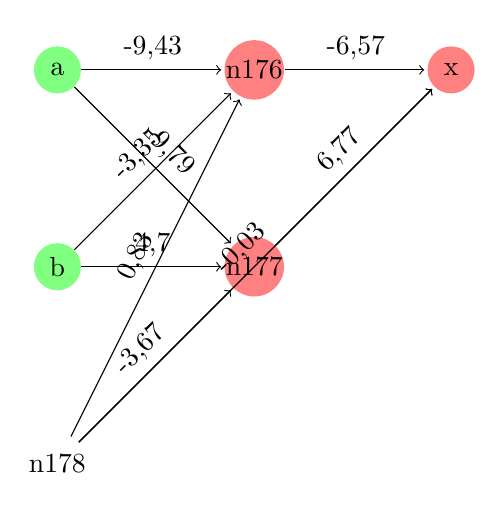
\begin{tikzpicture}[shorten >=1pt,->,draw=black!,node distance=2.5cm]
\tikzstyle{neuron}=[circle,fill=black!25,minimum size=17pt,inner sep=0pt]
\tikzstyle{constant}=[neuron, fill=white!50];
\tikzstyle{sigmoid}=[neuron, fill=red!50];
\tikzstyle{identity}=[neuron, fill=green!50];
\node [identity] (a) {a};
\node [identity,below of=a] (b) {b};
\node [constant,below of=b] (n178) {n178};
\node [sigmoid,right of=a] (n176) {n176};
\node [sigmoid,below of=n176] (n177) {n177};
\node [sigmoid,right of=n176] (x) {x};
\path[every node/.style={sloped,anchor=south,auto=false}]
(n176) edge node {-6,57} (x)
(n177) edge node {6,77} (x)
(a) edge node {-9,79} (n177)
(a) edge node {-9,43} (n176)
(b) edge node {-3,35} (n176)
(b) edge node {4,7} (n177)
(n178) edge node {-3,67} (n177)
(n178) edge node {0,83} (n176)
(n178) edge node {-0,03} (x)
;\end{tikzpicture}
\end{document}